\chapter{Some Theoretical Analysis}

\section{Analytical Solution} \label{sec:2.1}
The derivation of the analytical solution.

\subsection{Some Distributions}
Some derivations
\begin{align}
    \phi(x,y,z) = \phi_0 X(x) Y(y) Z(z)
\end{align}
where
\begin{subequations}
    \label{eq2.2}
    \begin{align}
        X(x) &= \cos \left(\frac{\pi x}{a}+\frac{\pi}{b}\right) \\
        Y(x) &= \cos \left(\frac{\pi y}{c}\right) \\
        Z(x) &= \cos \left(\frac{\pi z}{d}\right)         
    \end{align}
\end{subequations}
The coordinates in Eq.(\ref{eq2.2}) are in units of inch and the origin is at the core center.
The coolant in the core flows downward so the $z$-direction flux distribution is of the greatest 
interest in making a model that represents heat transfer in the coolant channel.

\subsection{Other Distributions}
Similar derivations.


\section{Numerical Simulation}

Some simulations.

Insert a EPS vector figure (see Fig. \ref{fig:eps_figure}).
\begin{figure}[!htbp]
    \captionsetup{name={Fig. }}
    \centering
    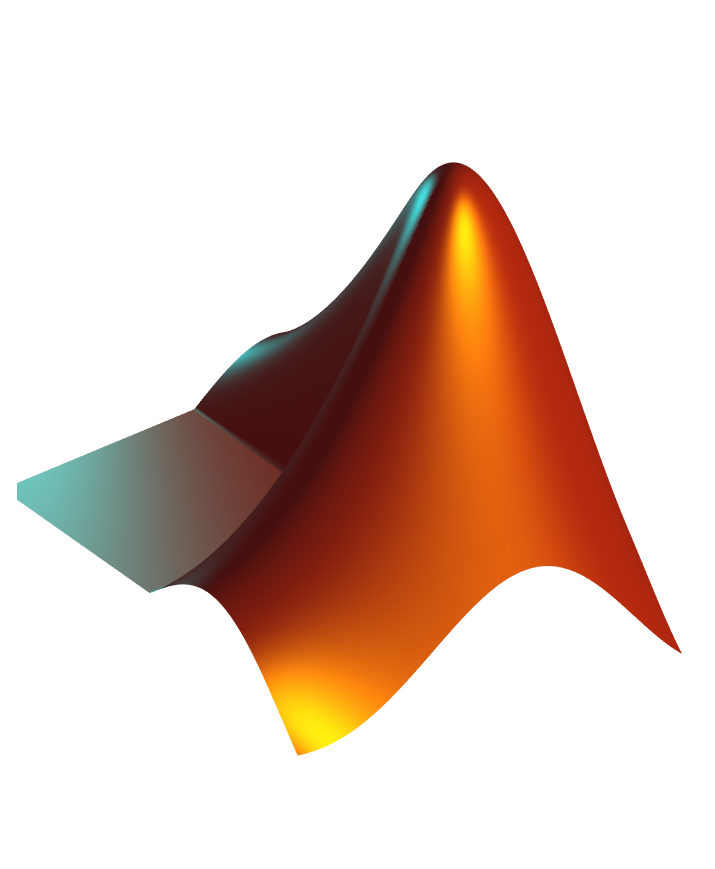
\includegraphics[width=0.5\textwidth]{fig/matlab-logo.eps}
    \caption{A vector figure}
    \label{fig:eps_figure}
\end{figure}